\documentclass{beamer}
\usepackage[MeX]{polski} 
\title{Fotosynteza}
\author{Magdalena Smoczyńska}
\institute{Uniwersytet Gdański}
\date{2023}
\usetheme{Boadilla}
\usecolortheme{rose}
\graphicspath{ {./images/} }
\usepackage{adjustbox}
\renewcommand{\footnotesize}{\tiny} 

\begin{document}
	
	\frame{\titlepage}
	\begin{frame}
		\frametitle{Spis tresci}
		\tableofcontents
	\end{frame}

\section{Informacje}
	\begin{frame}
		\frametitle{Definicja}
		Fotosynteza jest skomplikowanym procesem biochemicznym i fizjologicznym, charakterystycznym dla fotoautotrofów. Polega na asymilacji CO2 przy udziale energii świetlnej, co pozwala na utworzenie własnych związków organicznych. Fotosyntezę dzieli się na:
		\begin{enumerate}
			\item Faza jasna
			\item Faza ciemna (cykl Calvina)
		\end{enumerate}
		 Jest to proces przeprowadzany przez rośliny zielone, niektóre protisty, sinice i bakterie.
	\end{frame}

\section{Faza jasna}
	\begin{frame}{Faza jasna}
		Faza jasna zależy od światła i pozwala na utworzenie siły asymilacyjnej w postaci ATP i NADPH, wykorzystywanej następnie w reakcjach fazy ciemnej. Faza jasna zachodzi w błonach tylakoidów gran chloroplastów. Aby możliwe było wykorzystanie energii świetlnej i jej zamiana w energię użyteczną biologicznie, konieczne są cząsteczki zdolne do absorpcji światła. Takimi cząsteczkami są barwniki fotosyntetyczne.
		\begin{table}
			\hfill
		\begin{tabular}{|c||c|}
			\hline
			chlorofil a & chlorofil b \\ 
			\hline
			niebieski & żółty\\ 
			\hline
			CH3 przyłączony & CHO przyłączony\\ 
			\hline
		\end{tabular}
		\end{table}
	\end{frame}

\section{Faza jasna}
	\begin{frame}
		\frametitle{Fotosystemy}
			Cząsteczki barwników fotosyntetycznych tworzą uporządkowane struktury – fotoukłady (fotosystemy). Ze względu na różnice w budowie centrum reakcji wyróżnia się dwa rodzaje fotosystemów
		\begin{columns}[t]
			\begin{column}{.5\textwidth}
				\adjincludegraphics[width=.8\linewidth, valign=t]{faza_jasna.jpg}
				\label{fig: faza jasna}
			\end{column}
			\begin{column}{.5\textwidth}
				\\\begin{itemize}
					\item Fotosystem I
					\item Fotosystem
				\end{itemize}
			\end{column}
		\end{columns}
	\end{frame}

\section{Faza jasna}
	\begin{frame}
		\frametitle{Przebieg}
		Pod wpływem światła PSI ulega wzbudzeniu i zostają z niego wybite elektrony. Po odebraniu przez pierwotny akceptor elektronów wędrują one przenośnikami, aż trafiają na cząsteczkę NADP+, która ulega zredukowaniu do NADPH. W PSI brakuje elektronów. PSII jest pobudzony przez światło i PSI zasysa od niego elektrony. Wówczas w PSII brakuje elektronów i zostają one uzupełnione bezpośrednio z wody – zachodzi fotoliza, czyli rozpad wody w świetle na 2 elektrony, 2 H+ oraz ½ O2, uwalniany do atmosfery. Cały ten proces nazywany jest niecyklicznym transportem elektronów.
		\begin{figure}[H]
			\centering
			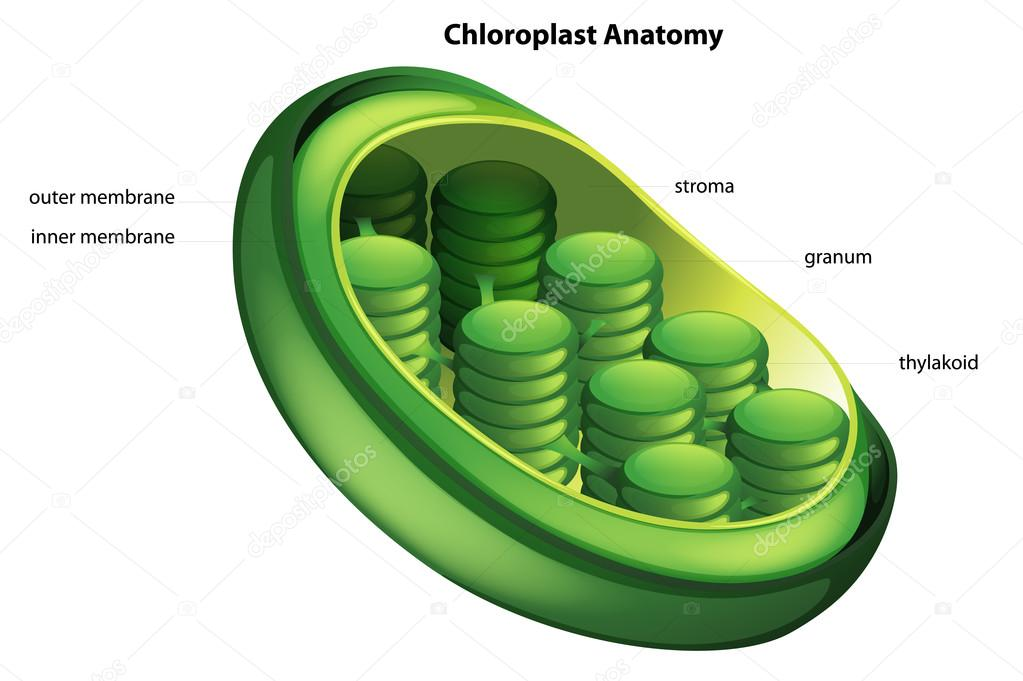
\includegraphics[width=5cm, height=3cm]{chloroplast.jpg}
			\caption{chloroplast}
			\label{fig: chloroplast}
		\end{figure}
		Powstaje różnica potencjałów – po zewnętrznej stonie błony tylakoidu tworzy się niedobór protonów, a we wnętrzu nadmiar. Jony H+ wracają do stromy przez specjalne kanały jonowe, a ich energia kinetyczna zamieniana jest w ruch obrotowy innych białek, co umożliwia syntezę i uwolnienie cząsteczek ATP. Cały proces nazywany jest fosforylacją fotosyntetyczną niecykliczną.
	\end{frame}

\section{Faza ciemna}
	\begin{frame}
		\frametitle{Zwiazki}
			\begin{columns}[t]
				\begin{column}{.5\textwidth}
					\\\adjincludegraphics[width=.8\linewidth, valign=t]{rubp.png}
					\newline
					\label{fig: rubp}
				\end{column}
				\begin{column}{.5\textwidth}
					\begin{enumerate}
						\item aldehyd 3-fosfoglicerynowy
						\item rybulozobifosforan
						\item kwas 3-fosfoglicerynowy
					\end{enumerate}
				\end{column}
			\end{columns}
			 Odniesienie do zdjecia ~\ref{fig: chloroplast}
	\end{frame}


\begin{frame}{Etapy}
\begin{columns}[T]
	\column{0.99\textwidth}
	\begin{itemize}
		\item Faza karboksylacji
		\item Faza redukcji
		\item Faza regeneracji
	\end{itemize}
	
	\column{0.01\textwidth}
	\hspace*{-5cm}
	\includegraphics[width=5cm]{cykl_calvina.jpg}
\end{columns}
\end{frame}


\begin{frame}{Przebieg}
Karboksylacja katalizowana jest przez enzym Rubisco i polega na przyłączeniu CO2 do pięciowęglowego RuBP – rybulozo-1,5-bifosforanu. W wyniku tego procesu powstaje sześciowęglowa cząsteczka, która rozpada się na dwie trójwęglowe cząsteczki PGA – kwasu 3-fosfoglicerynowego. W kolejnym etapie – redukcji – dochodzi do aktywacji PGA, a następnie jego redukcji do PGAL (aldehydu 3-fosfoglicerynowego). Do tego etapu wykorzystywane są NADPH i ATP, utworzone w fazie jasnej fotosyntezy. Ostatni etap cyklu Calvina to regeneracji, czyli odtworzenie pięciowęglowego akceptora CO2, do czego wykorzystywana jest większość cząsteczek PGAL.
	\begin{columns}
		\column{0.01\textwidth}
		\begin{figure}
			\hspace*{-3cm}
			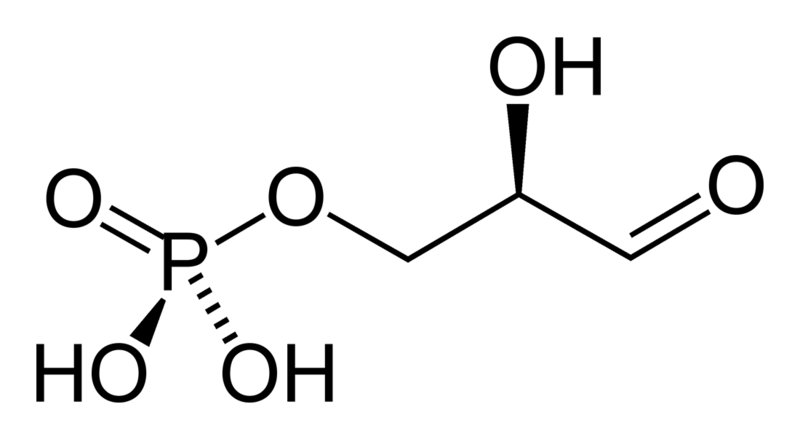
\includegraphics[width=4cm]{pgal.png}
		\end{figure}
		
		\column{0.01\textwidth}

	\end{columns}
\end{frame}

\section{Źródła}
\begin{frame}{Bibliografia}
\begin{thebibliography}{10}
	\bibitem{Office}matura100procent ``fotosynteza," \emph{przebieg fotosyntezy faza jasna i ciemna}, pp. 201, October 2021.
\end{thebibliography}
\end{frame}



\end{document}